% !TEX root = ../presentation.tex
% !BIB program = biber
% !TEX program = xelatex

\section[A Retrospective Study on Machine Learning-Assisted Stroke Recognition for Medical Helpline Calls]{a retrospective study on machine learning-assisted stroke recognition\\ for medical helpline calls}


\begin{frame}
    \frametitle{Stroke}
    \begin{itemize}
        \item Stroke is a leading cause of \highlight{disability and death} worldwide \parencite{cite1,cite2,cite3}.
        \item Effective treatment is very \highlight{time-sensitive}. \parencite{cite4,cite5}.
        \item The gateway to \highlight{ambulance transport and hospital admittance} is through \highlight{prehospital telehealth services}.
        \item \highlight{Mobile stroke units} has made it possible to deliver advanced treatment faster \parencite{cite6,cite7}.
        \item The effectiveness of mobile stroke units hinges on \highlight{call-taker recognition of stroke} \parencite{cite6,cite7}.
        \item But stroke 
    \end{itemize}
\end{frame}


\begin{frame}
    \frametitle{The study}
    \begin{itemize}
        \item Collaboration between \highlight{Corti} and the \highlight{Copenhagen Emergency Medical Services (CEMS)} (``Region Hovedstadens Akutberedskab").
        \item CEMS provides prehospital telehealth services in the Capital Region of Denmark (1.9M people).
        \item CEMS operates the 1-1-2 emergency line (similar to 9-1-1) and the 1813 medical helpline (non-life-threatening conditions when general practitioner is unavailable).
        \item Approximately half of all patients with stroke do not receive the correct triage for their condition from call-takers \parencite{cite10,cite11,cite12}. 
        \vspace{1em}
        \item We wanted to investigate if a machine learning model could assist call-takers of 1813 in recognizing stroke.
    \end{itemize}
\end{frame}


\begin{frame}
    \frametitle{Population selection and datasets}
    \begin{figure}
        \centering
        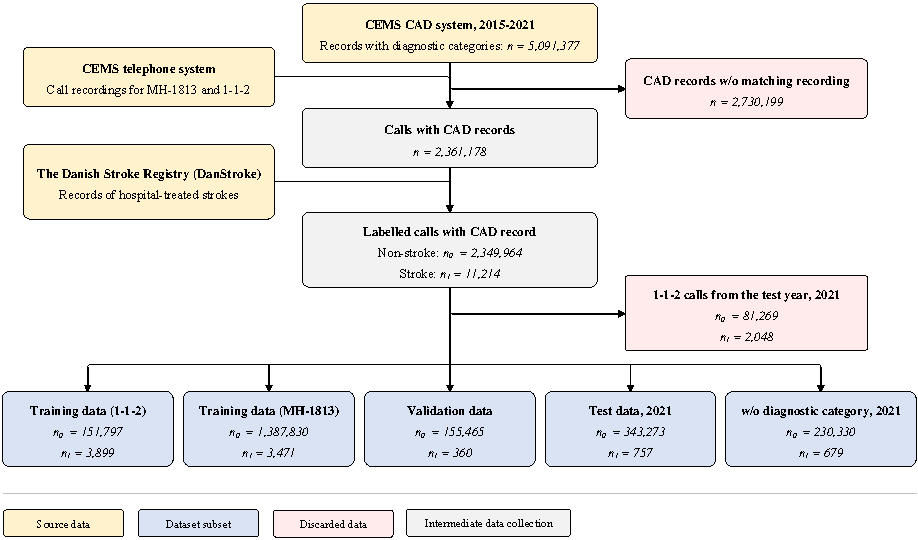
\includegraphics[width=0.65\paperwidth]{../graphics/paper_retrospective/data_flowchart.pdf}
        % \caption{Overview of data flow from the initial data sources to the final stroke dataset.}
    \end{figure}
\end{frame}


\newcommand{\verticalmultirow}[2]{\parbox[t]{3mm}{\multirow{#1}{*}{\rotatebox[origin=c]{90}{#2}}}}
\begin{frame}
    \frametitle{Population characteristics}
    \begin{table}[t]
        \centering
        % \caption{Population characteristics for each data subset.}
        % \label{tab_retrospective:table1-population-characteristics}
        \resizebox*{0.98\textwidth}{!}{%
        \begin{tabular}{l|l|ccccc}
            \toprule
            &                      & Training (112) & Training (MH-1813) & Validation & Test & 2021 w/o category \\

            \midrule
            \verticalmultirow{5}{\emph{All calls}}    & Num. calls   & 155,696 & 1,391,301 & 155,825 & 344,030 & 231,009 \\
                                                                     & Female                & 74,640 (47.94\%) & 792,783 (56.98\%) & 86,959 (55.81\%) & 190,974 (55.51\%) & 134,324 (58.14\%) \\
                                                                     & Male                  & 79,564 (51.10\%) & 596,760 (42.89\%) & 68,866 (44.19\%) & 153,050 (44.49\%) & 96,258 (41.67\%) \\
                                                                     & 65+ years             & 72,930 (46.84\%) & 335,146 (24.09\%) & 30,313 (19.45\%) & 65,652 (19.08\%) & 81,488 (35.27\%) \\
                                                                     & Age (mean $\pm$ std.) & 59.47 ± 21.24 & 47.12 ± 21.38 & 44.63 ± 20.08 & 44.31 ± 20.10 & 50.36 ± 22.77 \\

            \midrule
            \verticalmultirow{5}{\emph{Stroke calls}} & Num. calls   & 3,899 & 3,471 & 360 & 757 & 679 \\
                                                                     & Female                & 1,784 (45.76\%) & 1,654 (47.65\%) & 161 (44.72\%) & 349 (46.10\%) & 366 (53.90\%) \\
                                                                     & Male                  & 2,115 (54.24\%) & 1,815 (52.29\%) & 199 (55.28\%) & 408 (53.90\%) & 313 (46.10\%) \\
                                                                     & 65+ years             & 2,968 (76.12\%) & 2,421 (69.75\%) & 250 (69.44\%) & 555 (73.32\%) & 567 (83.51\%) \\
                                                                     & Age (mean $\pm$ std.) & 72.91 ± 12.77 & 70.68 ± 13.85 & 70.93 ± 13.83 & 71.51 ± 13.41 & 73.41 ± 14.11 \\

            \midrule
            \verticalmultirow{5}{\emph{Non-stroke}}   & Num. calls   & 151,797 & 1,387,830 & 155,465 & 343,273 & 230,330 \\
                                                                     & Female                & 72,856 (48.00\%) & 791,129 (57.00\%) & 86,798 (55.83\%) & 190,625 (55.53\%) & 133,958 (58.16\%) \\
                                                                     & Male                  & 77,449 (51.02\%) & 594,945 (42.87\%) & 68,667 (44.17\%) & 152,642 (44.47\%) & 95,945 (41.66\%) \\
                                                                     & 65+ years             & 69,962 (46.09\%) & 332,725 (23.97\%) & 30,063 (19.34\%) & 65,097 (18.96\%) & 80,921 (35.13\%) \\
                                                                     & Age (mean $\pm$ std.) & 59.12 ± 21.30 & 47.06 ± 21.36 & 44.57 ± 20.05 & 44.25 ± 20.08 & 50.29 ± 22.76 \\

            \bottomrule
        \end{tabular}%
        }
    \end{table}
\end{frame}


% \begin{frame}
%     \frametitle{Population characteristics}
%     \begin{table}[t]
%         \centering
%         % \caption{Population characteristics for each data subset.}
%         % \label{tab_retrospective:table1-population-characteristics}
%         \resizebox*{0.98\textwidth}{!}{%
%         \begin{tabular}{l|ccccc}
%             \toprule
%                                   & Training (112) & Training (MH-1813) & Validation & Test & 2021 w/o category \\

%             \midrule
%             \multicolumn{6}{c}{\emph{All calls}} \\
%             \midrule
%             Num. calls            & 155,696 & 1,391,301 & 155,825 & 344,030 & 231,009 \\
%             Female                & 74,640 (47.94\%) & 792,783 (56.98\%) & 86,959 (55.81\%) & 190,974 (55.51\%) & 134,324 (58.14\%) \\
%             Male                  & 79,564 (51.10\%) & 596,760 (42.89\%) & 68,866 (44.19\%) & 153,050 (44.49\%) & 96,258 (41.67\%) \\
%             65+ years             & 72,930 (46.84\%) & 335,146 (24.09\%) & 30,313 (19.45\%) & 65,652 (19.08\%) & 81,488 (35.27\%) \\
%             Age (mean $\pm$ std.) & 59.47 ± 21.24 & 47.12 ± 21.38 & 44.63 ± 20.08 & 44.31 ± 20.10 & 50.36 ± 22.77 \\

%             \midrule
%             \multicolumn{6}{c}{\emph{Stroke calls}} \\
%             \midrule
%             Num. calls            & 3,899 & 3,471 & 360 & 757 & 679 \\
%             Female                & 1,784 (45.76\%) & 1,654 (47.65\%) & 161 (44.72\%) & 349 (46.10\%) & 366 (53.90\%) \\
%             Male                  & 2,115 (54.24\%) & 1,815 (52.29\%) & 199 (55.28\%) & 408 (53.90\%) & 313 (46.10\%) \\
%             65+ years             & 2,968 (76.12\%) & 2,421 (69.75\%) & 250 (69.44\%) & 555 (73.32\%) & 567 (83.51\%) \\
%             Age (mean $\pm$ std.) & 72.91 ± 12.77 & 70.68 ± 13.85 & 70.93 ± 13.83 & 71.51 ± 13.41 & 73.41 ± 14.11 \\

%             \midrule
%             \multicolumn{6}{c}{\emph{Non-stroke calls}} \\
%             \midrule
%             Num. calls            & 151,797 & 1,387,830 & 155,465 & 343,273 & 230,330 \\
%             Female                & 72,856 (48.00\%) & 791,129 (57.00\%) & 86,798 (55.83\%) & 190,625 (55.53\%) & 133,958 (58.16\%) \\
%             Male                  & 77,449 (51.02\%) & 594,945 (42.87\%) & 68,667 (44.17\%) & 152,642 (44.47\%) & 95,945 (41.66\%) \\
%             65+ years             & 69,962 (46.09\%) & 332,725 (23.97\%) & 30,063 (19.34\%) & 65,097 (18.96\%) & 80,921 (35.13\%) \\
%             Age (mean $\pm$ std.) & 59.12 ± 21.30 & 47.06 ± 21.36 & 44.57 ± 20.05 & 44.25 ± 20.08 & 50.29 ± 22.76 \\

%             \bottomrule
%         \end{tabular}%
%         }
%     \end{table}
% \end{frame}



\begin{frame}
    \frametitle{Model design}
    \begin{figure}
        \centering
        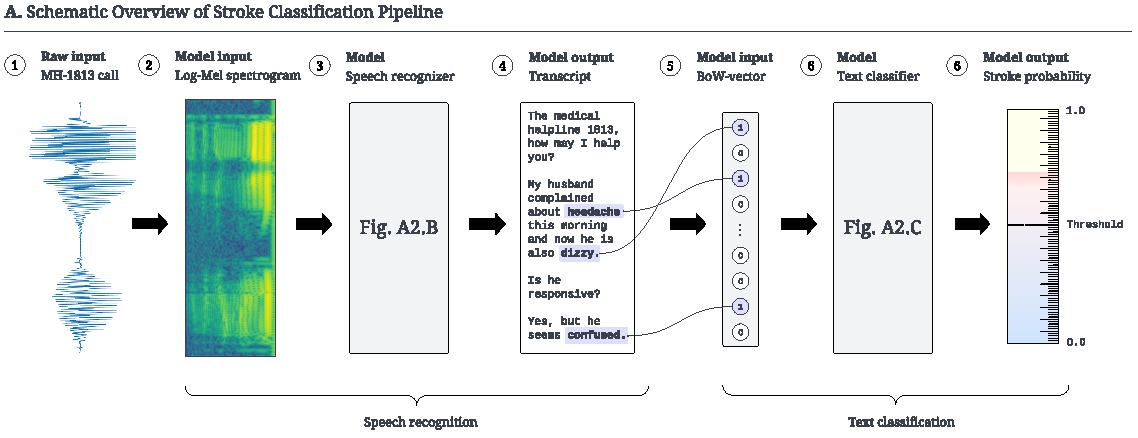
\includegraphics[width=0.90\paperwidth]{../graphics/paper_retrospective/model_sketch-top-part.pdf}
    \end{figure}
\end{frame}


\begin{frame}
    \frametitle{Model design}
    \begin{figure}
        \centering
        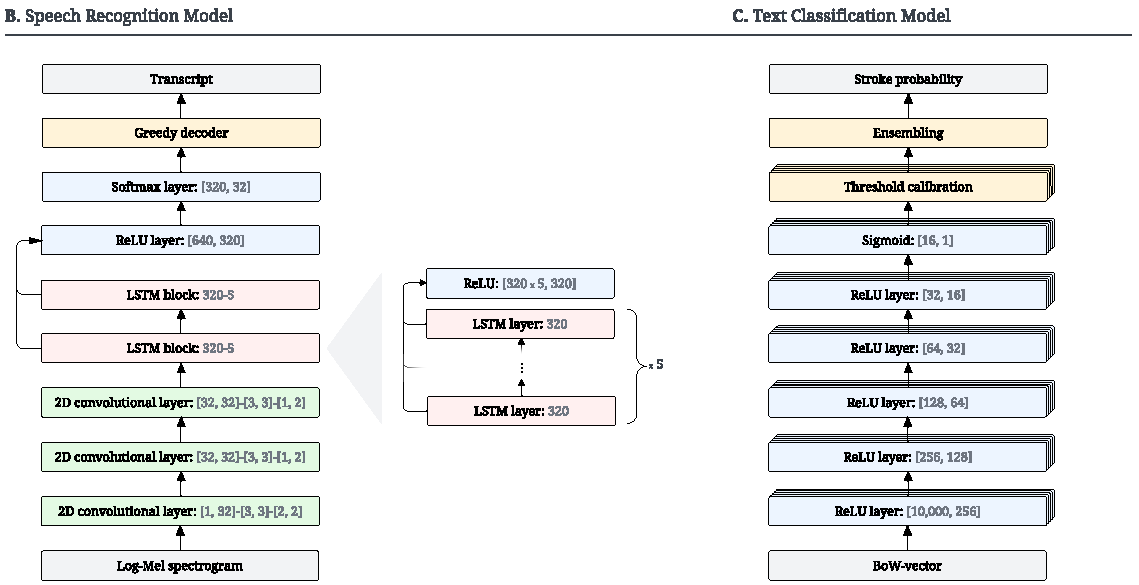
\includegraphics[width=0.70\paperwidth]{../graphics/paper_retrospective/model_sketch-bottom-part.pdf}
    \end{figure}
\end{frame}


\newcommand{\shade}[1]{{\color{black!40}#1}}

\begin{frame}
    \frametitle{Main results}
    \begin{table}[t]
        \centering
        \caption{MH-1813 test set performance in demographic subgroups (age/sex) [mean (95\% CI)]}
        \label{tab_retrospective:table2-main-results}
        \resizebox*{0.98\textwidth}{!}{%
        \begin{tabular}{ll|ccccc}
            \toprule
            Subset & Predictor & F1-score [\%] $\uparrow$ & Sensitivity [\%] $\uparrow$ & PPV [\%] $\uparrow$ & \makecell{FOR [\%] $\downarrow$ \\ (1 - specificity)} & \makecell{FPR [\%] $\downarrow$ \\ (1 - NPV)} \\
    
            % \midrule
            % \multicolumn{6}{c}{\emph{Overall}} \\
            \midrule
            \emph{Overall} & Call-takers                                 & 25.8 \shade{(23.7-27.9)} & 52.7 \shade{(49.2-56.4)} & 17.1 \shade{(15.5-18.6)} & 0.105 \shade{(0.094-0.116)} & 0.565 \shade{(0.539-0.590)} \\
            & Model                                       & 35.7 \shade{(35.0-36.4)} & 63.0 \shade{(62.0-64.1)} & 24.9 \shade{(24.3-25.5)} & 0.082 \shade{(0.079-0.085)} & 0.419 \shade{(0.413-0.426)} \\
            % \makecell[l]{Model \\ w/o 1-1-2 training data} & 32.4 \shade{(31.8-33.1)} & 60.4 \shade{(59.3-61.4)} & 22.2 \shade{(21.6-22.7)} & 0.088 \shade{(0.085-0.091)} & 0.467 \shade{(0.460-0.474)} \\
            % \midrule
    
            % \midrule
            % \multicolumn{6}{c}{\emph{Without 112 training data}} \\
            % \midrule
            % Model       & 32.4 \shade{(31.8-33.1)} & 60.4 \shade{(59.3-61.4)} & 22.2 \shade{(21.6-22.7)} & 0.088 \shade{(0.085-0.091)} & 0.467 \shade{(0.460-0.474)} \\
    
            % \midrule
            % \multicolumn{6}{c}{\emph{On MH-1813 data without diagnostic category}} \\
            % \midrule
            % Model                                       & 32.6 \shade{(31.9-33.4)} & 48.3 \shade{(47.2-49.4)} & 24.7 \shade{(23.9-25.3)} & 0.153 \shade{(0.148-0.158)} & 0.435 \shade{(0.427-0.443)} \\
    
            % \midrule
            % \multicolumn{6}{c}{\emph{18-64 years}} \\
            \midrule
            \emph{18-64 years} & Call-takers                                 & 15.9 \shade{(13.1-18.5)} & 50.5 \shade{(43.6-57.2)} & 9.40 \shade{(7.61-11.2)} & 0.036 \shade{(0.028-0.043)} & 0.353 \shade{(0.331-0.375)} \\
            & Model                                       & 22.9 \shade{(21.8-24.0)} & 54.1 \shade{(52.1-56.3)} & 14.5 \shade{(13.8-15.3)} & 0.033 \shade{(0.031-0.035)} & 0.231 \shade{(0.226-0.236)} \\ 
    
            % \midrule
            % \multicolumn{6}{c}{\emph{65+ years}} \\
            \midrule
            \emph{65+ years} & Call-takers                                 & 32.9 \shade{(30.1-35.7)} & 53.5 \shade{(49.4-57.6)} & 23.7 \shade{(21.4-26.0)} & 0.401 \shade{(0.352-0.449)} & 1.467 \shade{(1.373-1.560)} \\
            & Model                                       & 42.8 \shade{(41.9-43.7)} & 66.3 \shade{(65.1-67.5)} & 31.6 \shade{(30.8-32.4)} & 0.290 \shade{(0.278-0.303)} & 1.224 \shade{(1.198-1.249)} \\
    
            % \midrule
            % \multicolumn{6}{c}{\emph{Male}} \\
            \midrule
            \emph{Male} & Call-takers                                 & 30.2 \shade{(27.2-33.3)} & 53.9 \shade{(49.1-58.9)} & 21.0 \shade{(18.5-23.5)} & 0.124 \shade{(0.105-0.141)} & 0.542 \shade{(0.506-0.580)} \\
            & Model                                       & 39.0 \shade{(38.0-40.1)} & 63.7 \shade{(62.3-65.2)} & 28.1 \shade{(27.3-29.0)} & 0.097 \shade{(0.093-0.102)} & 0.435 \shade{(0.425-0.445)} \\
    
            % \midrule
            % \multicolumn{6}{c}{\emph{Female}} \\
            \midrule
            \emph{Female} & Call-takers                                 & 21.9 \shade{(19.1-24.6)} & 51.3 \shade{(46.0-56.6)} & 13.9 \shade{(12.0-15.8)} & 0.090 \shade{(0.076-0.103)} & 0.582 \shade{(0.547-0.616)} \\
            & Model                                       & 32.4 \shade{(31.4-33.4)} & 62.3 \shade{(60.7-63.8)} & 21.9 \shade{(21.1-22.7)} & 0.069 \shade{(0.066-0.073)} & 0.407 \shade{(0.399-0.416)} \\
            
            \bottomrule
        \end{tabular}%
        }
    \end{table}
    % \begin{figure}
    %     \centering
    %     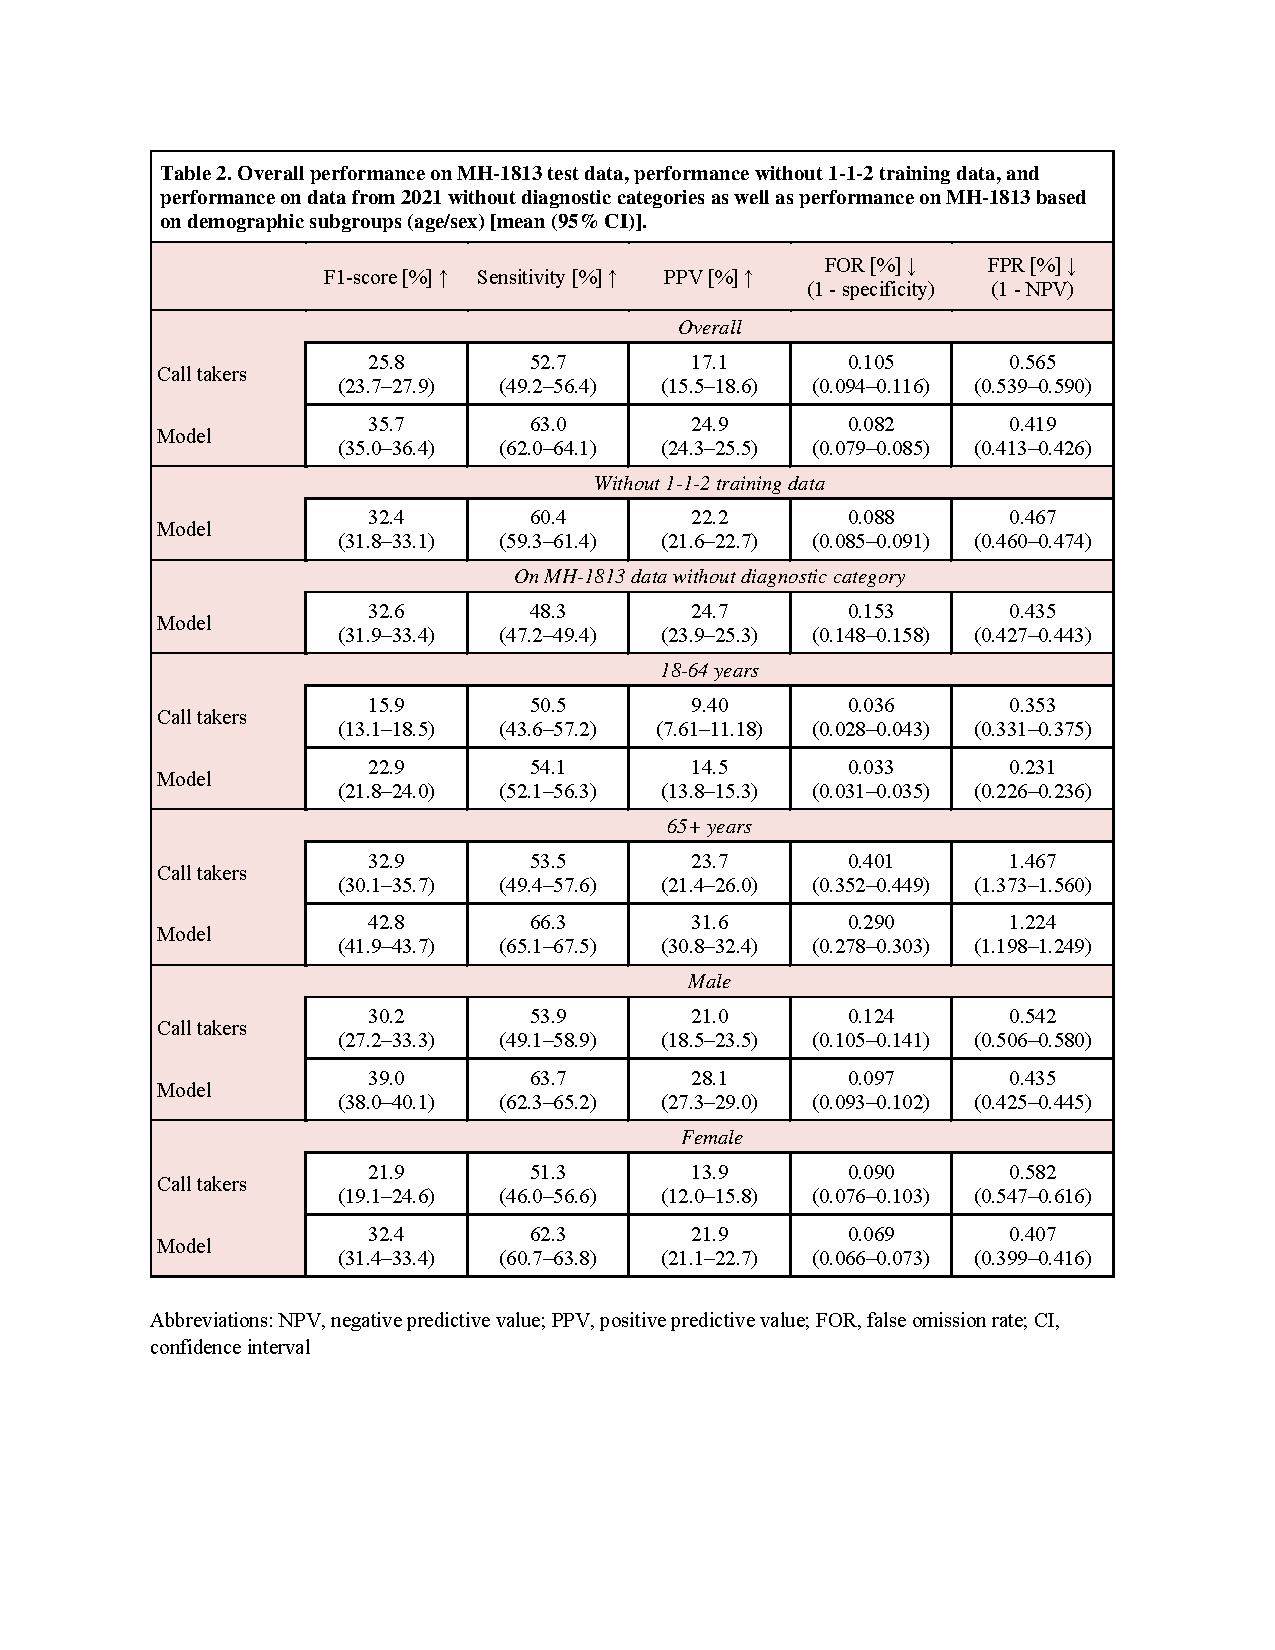
\includegraphics[width=0.3\paperwidth]{../graphics/paper_retrospective/table2.pdf}
    % \end{figure}
\end{frame}


\begin{frame}
    \frametitle{Model performance}
    \begin{figure}
        \centering
        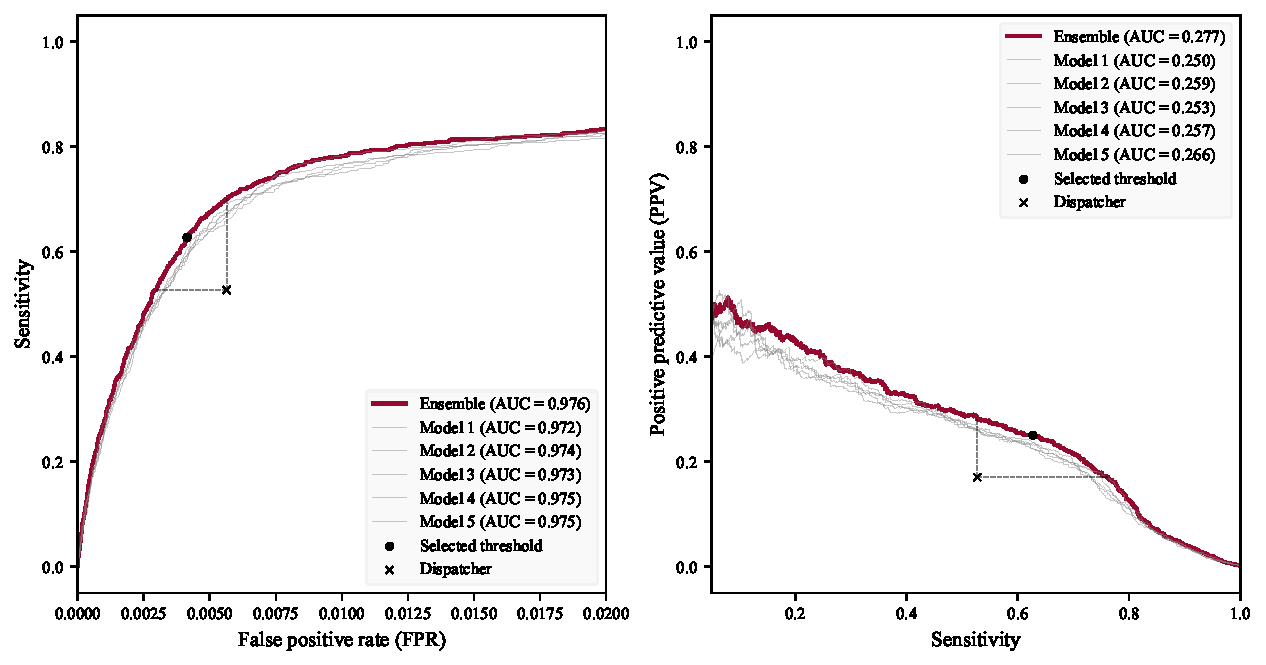
\includegraphics[width=0.65\paperwidth]{../graphics/paper_retrospective/figure1.pdf}
        \caption{Left, the ROC curve and, right, PPV-sensitivity curve (precision-recall curve). Models 1-5 are the individual models that make up the ensemble model.}
    \end{figure}
\end{frame}


\begin{frame}
    \frametitle{Model performance}
    \begin{figure}
        \centering
        \caption{Confusion matrices of predictions for call takers and the model on the test set. Numbers for the model are given as the rounded mean over eleven runs.}
        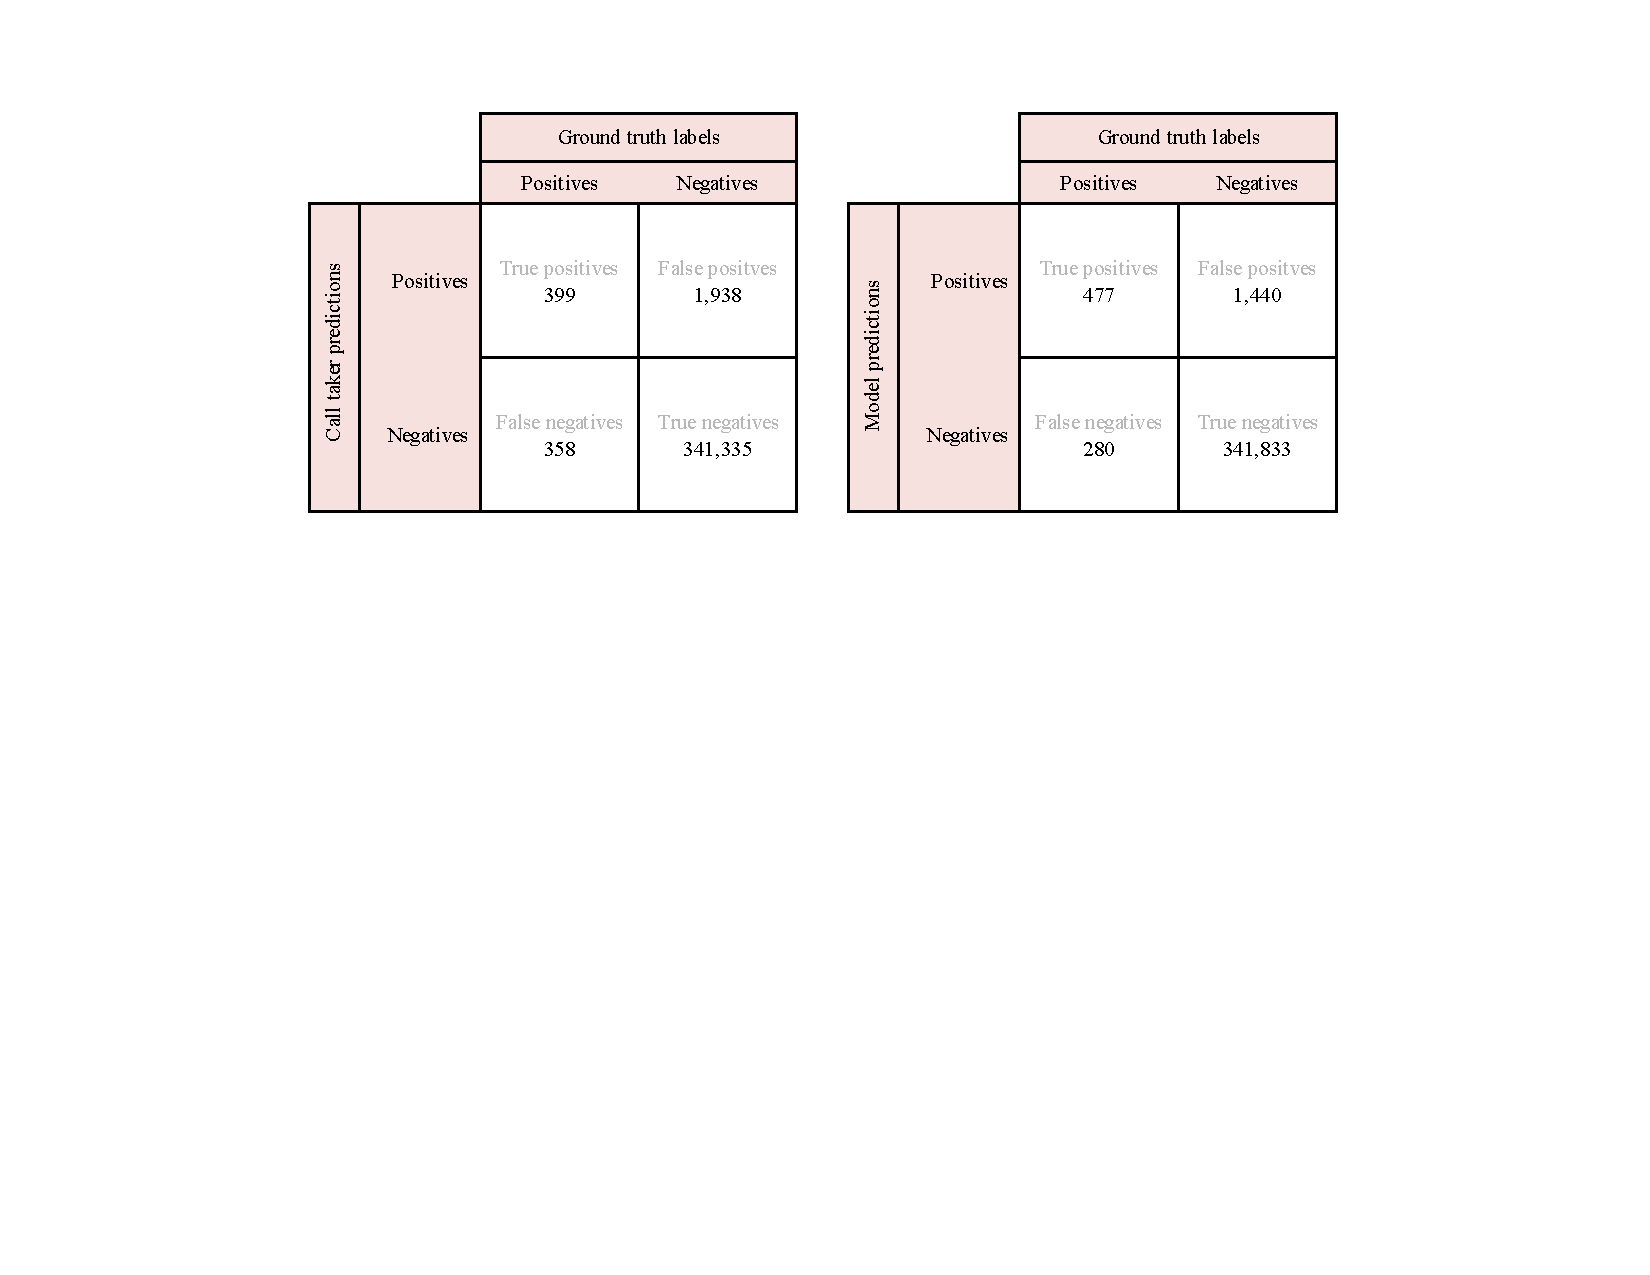
\includegraphics[width=0.85\paperwidth]{../graphics/paper_retrospective/figure2.pdf}
    \end{figure}
\end{frame}


\begin{frame}
    \frametitle{Which features are important?}
    Let $z^{(n, d, w)}$ be the logit output of model $n$ in the ensemble for transcript $d$ when the word $w$ is occluded. For transcript $d$, we computed the word impact score $i^{(d, w)}$ as the mean difference between the logit before and after occlusion.
    %
    \begin{equation}
        i^{(d,w)} = \frac{1}{N_d} \sum_{n=1}^{N_d} \left( z^{(n, d)} - z^{(n, d, w)} \right) \enspace .
    \end{equation}
    %
    To select words for inspection, we computed a word-rank score, $r^{(w)}$, as the sum of the signed squares of the impact:
    %
    \begin{equation}
        r^{(w)} = \sum_{d=1}^{N} \text{sign}\left( i^{(d, w)} \right) \left( i^{(d,w)}\right) ^2 \enspace .
    \end{equation}
    %
    Squaring $i^{(d,w)}$ favors rare features with a high impact over common features with a low impact.
\end{frame}


\begin{frame}
    \frametitle{Which features are important?}
    \begin{table}[t]
        \centering
        % \caption[Words with the largest positive and negative ranking score in calls predicted as stroke and non-stroke, respectively.]{English translation of words with the largest positive and negative ranking score in calls predicted as stroke and non-stroke, respectively. For this analysis, we used the model with the median F1-score out of 11 randomly seeded runs.}
        % \label{tab_retrospective:table3-occlusion-analysis}
        \resizebox*{0.98\textwidth}{!}{%
        \begin{tabular}{l|lr|lr}
            \toprule
                        & \multicolumn{2}{c|}{Positive ranking score, $r^{(w)}$} & \multicolumn{2}{c}{Negative ranking score, $r^{(w)}$} \\
            \midrule
                        & \multicolumn{2}{c|}{Stroke predictions, $D=1,897$} & \multicolumn{2}{c}{Non-stroke predictions, $D=342,133$} \\
            \midrule
                        & Word, $w$ \textit{(translated)} & Occurrences, $D^{(w)}$ & Word, $w$ \textit{(translated)} & Occurrences, $D^{(w)}$ \\
            \midrule
            1.  & Ambulance & 1,680 & Tetanus & 4,378 \\        
            2.  & Blood clot & 895 & Pregnant & 8,749 \\        
            3.  & Left & 1,108 & Cut & 7,592 \\        
            4.  & Right & 1,050 & Bandage & 4,561 \\        
            5.  & Double vision & 84 & Amager (a location) & 23,776 \\        
            6.  & The words & 344 & O'clock & 94,436 \\        
            7.  & Suddenly & 783 & The emergency room & 42,809 \\        
            8.  & Arm & 709 & The police & 2,903 \\        
            9.  & Side & 1,139 & Swollen & 60,559 \\        
            10. & Stroke & 117 & Over the counter (OTC) & 4,641 \\        
            11. & Double & 113 & The neck & 30,151 \\        
            12. & Control & 134 & Fever & 112,586 \\        
            13. & Call & 39 & Prescription & 5,450 \\        
            14. & Numb & 94 & Centimeter & 12,026 \\        
            15. & Minutes & 763 & The knee & 8,875 \\        
            16. & Difficulties speaking & 44 & The pharmacy & 10,085 \\        
            17. & Hemorrhagic stroke & 133 & The stomach & 42,105 \\        
            18. & Hand & 297 & Psychiatric & 3,688 \\        
            19. & The ambulance & 521 & Pneumonia & 7,597 \\        
            20. & Slurred speech & 58 & Stomach pain & 10,551 \\        
            21. & Blood clots & 224 & Stool & 19,155 \\        
            22. & Fast & 663 & The ribs & 3,928 \\        
            23. & Express & 44 & Bleed & 10,501 \\        
            24. & Blood thinner & 259 & Bleeding & 24,313 \\        
            25. & Incoherent & 15 & Ribs & 2,941 \\        
            26. & Lopsided & 211 & Broken & 19,415 \\        
            27. & Reduced & 528 & Inflammation & 10,050 \\        
            28. & Hangs & 628 & Common cold & 8,127 \\        
            29. & Transient & 48 & Morning or morrow & 78,558 \\        
            30. & Not making sense & 14 & Swelling & 17,762 \\        
            \bottomrule
        \end{tabular}%
        }
    \end{table}
    % \begin{figure}
    %     \centering
    %     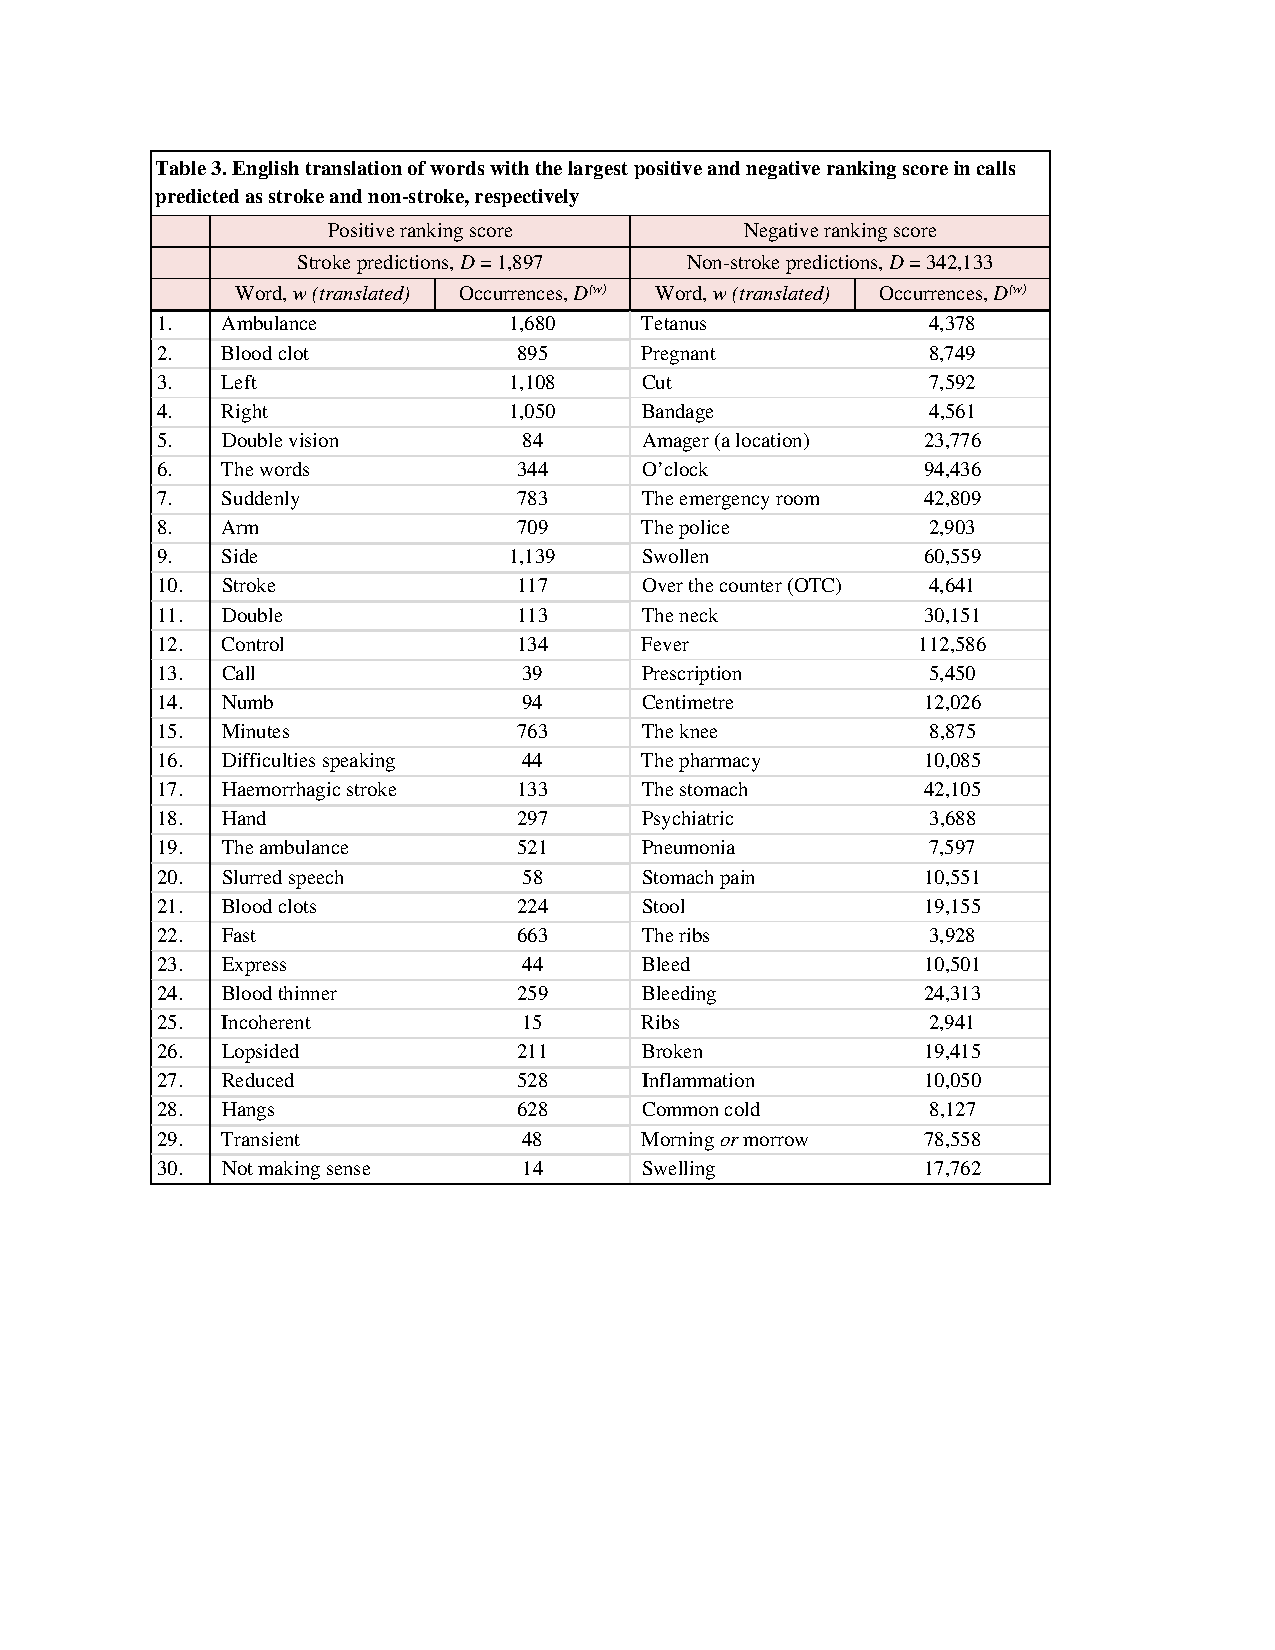
\includegraphics[width=0.4\paperwidth]{../graphics/paper_retrospective/table3.pdf}
    % \end{figure}
\end{frame}


\begin{frame}
    \frametitle{Simulated prospective study}
    \begin{enumerate}
        \item[I.] \highlight{When} is the model prediction presented to the call-taker?
        \begin{enumerate}
            \item[1.] Notify the call-taker \highlight{after the call ends}.
            \item[2.] Notify the call-taker \highlight{during the call}.
        \end{enumerate}
        \item[II.] \highlight{How} does prediction influence the diagnostic code the call-taker assigns to the call?
        \begin{enumerate}[label=\Alph*.]
            \item[A.] Call-takers \highlight{mirror model positives}.
            \item[B.] Call-takers \highlight{mirror model negatives}.
            \item[C.] Call-takers mirror model predictions (corresponds to main results of the model itself).
        \end{enumerate}
    \end{enumerate}
    \vspace{0.5em}
    To simulate the online scenario (2.), we \highlight{stream the transcript} to the model and make predictions every 50 words. 
    A stroke positive is triggered only when three consecutive positive predictions are made. 
    This is similar to the strategy implemented for a previous RCT on cardiac arrest \cite{cite15}.

        % %
        % Option 1 is identical to the method used in the main study. In option 2, predictions are made during the call based only on partial transcriptions. We implemented option 2 in such a manner that the model predicted every time 50 new words were transcribed and added to the transcript. A stroke positive was triggered only when three consecutive positive predictions were made (i.e., without intermediate negative stroke predictions). In other words, the sigmoid activation of the model had to remain above 0.5 for three consecutive predictions, for example, after 150, 200, and 250 words were transcribed.
        
        % As we can only assume how call takers are influenced by model predictions (II), precisely evaluating the hypothetical performance of call takers when supported by a machine learning framework is impossible. Furthermore, option 2 may influence the conversation, further complicating matters. Therefore, we report the results combining the call taker and the model under the following two assumptions:
        % %
\end{frame}


\begin{frame}
    \frametitle{Simulated prospective study}

    \begin{table}
        \centering
        % \caption{Overall performance of model, call-takers and simulated combinations of model and call-takers on MH-1813 test data.}
        % \label{tab_retrospective:tableA9}
        \resizebox*{0.98\textwidth}{!}{%
        \begin{tabular}{c|c|cc|cc|cc}
            \toprule
    
            \textbf{Predictor} & \textbf{Call-taker} & \multicolumn{2}{c|}{\textbf{Model}} & \multicolumn{4}{c}{\textbf{Call-taker supported by the model (simulated)}} \\
            \midrule
            \textbf{When} & \textbf{During call} & \textbf{After call} & \textbf{During call} & \textbf{After call} & \textbf{During call} & \textbf{After call} & \textbf{During call} \\
            \midrule
            \textbf{Method} & - & - & - & \textbf{neg $\rightarrow$ pos} & \textbf{neg $\rightarrow$ pos} & \textbf{pos $\rightarrow$ neg} & \textbf{pos $\rightarrow$ neg} \\
            \midrule
    
            \makecell[l]{\textbf{F1-score} [\%] $\uparrow$}                   & \makecell[c]{25.8 \\ (23.7-27.9)} & \makecell[c]{35.7 \\ (35.0-36.4)} & \makecell[c]{33.1 \\ (32.4-33.7)} & \makecell[c]{28.9 \\ (28.3-29.5)} & \makecell[c]{27.6 \\ (27.0-28.1)}  & \makecell[c]{33.3 \\ (32.5-34.1)}& \makecell[c]{32.7 \\ (31.8-33.5)} \\
            \midrule
            \makecell[l]{\textbf{Sensitivity} [\%] $\uparrow$}                & \makecell[c]{52.7 \\ (49.2-56.4)} & \makecell[c]{63.0 \\ (62.0-64.1)} & \makecell[c]{58.7 \\ (57.7-59.8)} & \makecell[c]{72.4 \\ (71.5-73.3)} & \makecell[c]{72.3 \\ (71.4-73.3)} & \makecell[c]{43.4 \\ (42.3-44.5)} & \makecell[c]{39.1 \\ (38.1-40.1)} \\
            \midrule
            \makecell[l]{\textbf{PPV} [\%] $\uparrow$}                        & \makecell[c]{17.1 \\ (15.5-18.6)} & \makecell[c]{24.9 \\ (24.3-25.5)} & \makecell[c]{23.0 \\ (22.5-23.6)} & \makecell[c]{18.0 \\ (17.6-18.4)} & \makecell[c]{17.0 \\ (16.7-17.4)} & \makecell[c]{27.0 \\ (26.3-27.8)} & \makecell[c]{28.1 \\ (27.3-28.9)} \\
            \midrule
            \makecell[l]{\textbf{FOR} [\%] $\downarrow$ \\ (1 - NPV)}         & \makecell[c]{0.105 \\ (0.094-0.116)} & \makecell[c]{0.082 \\ (0.079-0.085)} & \makecell[c]{0.091 \\ (0.088-0.094)} & \makecell[c]{0.061 \\ (0.059-0.064)} & \makecell[c]{0.061 \\ (0.059-0.064)} & \makecell[c]{0.125 \\ (0.121-0.129)} & \makecell[c]{0.134 \\ (0.131-0.138)} \\
            \midrule
            \makecell[l]{\textbf{FPR} [\%] $\downarrow$ \\ (1 - specificity)} & \makecell[c]{0.565 \\ (0.539-0.590)} & \makecell[c]{0.419 \\ (0.413-0.426)} & \makecell[c]{0.432 \\ (0.426-0.439)} & \makecell[c]{0.726 \\ (0.717-0.735)} & \makecell[c]{0.776 \\ (0.767-0.786)} & \makecell[c]{0.258 \\ (0.253-0.263)} & \makecell[c]{0.221 \\ (0.216-0.226)} \\
    
            \bottomrule
        \end{tabular}%
        }
    \end{table}

\end{frame}


\begin{frame}
    \frametitle{Fine-tuning a large language model}
    \begin{table}
        \centering
        % \caption[Overall performance on MH-1813 test data for a fine"=tuned BERT model.]{Overall performance on MH-1813 test data for the fine-tuned BERT model described in the revised discussion of the paper. Includes performance of the call-takers and the multi-layer perceptron (MLP) from the main manuscript for ease of comparison [mean (95\% CI)]. NPV: negative predictive value, PPV: positive predictive value, FOR: false omission rate, CI: confidence interval.}
        % \label{tab_retrospective:tableA8}
        \resizebox*{0.98\textwidth}{!}{%
        \begin{tabular}{l|ccccc}
            \toprule
            & F1-score [\%] $\uparrow$ & Sensitivity [\%] $\uparrow$ & PPV [\%] $\uparrow$ & \makecell[c]{FOR [\%] $\downarrow$ \\ (1 - NPV)} & \makecell[c]{FPR [\%] $\downarrow$ \\ (1 - specificity)} \\
            \midrule
            & \multicolumn{5}{c}{\textit{Overall}} \\
            \midrule
            
            Call-takers                             & \makecell[c]{25.8 \\ (23.7-27.9)} & \makecell[c]{52.7 \\ (49.2-56.4)} & \makecell[c]{17.1 \\ (15.5-18.6)} & \makecell[c]{0.105 \\ (0.094-0.116)} & \makecell[c]{0.565 \\ (0.539-0.590)} \\
            \midrule
            \makecell[l]{MLP}                       & \makecell[c]{35.7 \\ (35.0-36.4)} & \makecell[c]{63.0 \\ (62.0-64.1)} & \makecell[c]{24.9 \\ (24.3-25.5)} & \makecell[c]{0.082 \\ (0.079-0.085)} & \makecell[c]{0.419 \\ (0.413-0.426)} \\
            \midrule
            \makecell[l]{BERT \\ (fine-tuned)}      & \makecell[c]{33.8 \\ (31.5-36.2)} & \makecell[c]{57.5 \\ (53.9-60.9)} & \makecell[c]{23.9 \\ (21.9-25.9)} & \makecell[c]{0.094 \\ (0.084-0.104)} & \makecell[c]{0.403 \\ (0.381-0.424)} \\
     
            \bottomrule
        \end{tabular}%
        }
    \end{table}
\end{frame}


\begin{frame}
    \frametitle{Future work}
    \begin{itemize}
        \item Self-supervised learning directly from audio data.
        \item Investigate learning to defer to predict methods \cite{verma_calibrated_2022}.
    \end{itemize}
\end{frame}
